\documentclass[11pt,a4paper]{article}

% Packages Ecriture
\usepackage[T1]{fontenc}
\usepackage[utf8]{inputenc}
\usepackage[french]{babel}
\usepackage{lmodern}

\renewcommand{\familydefault}{\sfdefault} 
\renewcommand{\ttdefault}{lmtt} 
\usepackage{eurosym}
\usepackage[np]{numprint}

% Packages Mise en page
\usepackage{geometry} % Permet la mise en page
\geometry{lmargin=2cm,rmargin=2cm,tmargin=2cm,bmargin=1.5cm} % Choix format et  des marges
\usepackage{fancyhdr}
\usepackage{framed} % Création d'environnements
\usepackage[framed,thmmarks]{ntheorem} % Gestions des environnements theorem
\usepackage{lastpage}

\usepackage{amsmath,amssymb,makeidx}
\usepackage{enumerate}
\usepackage[normalem]{ulem}
\usepackage{fancybox,graphicx}
\usepackage{tabularx}
\usepackage{ulem}
\usepackage{dcolumn}
\usepackage{textcomp}
\usepackage{diagbox}
\usepackage{tabularx}
\usepackage{lscape}
\usepackage{pstricks,pst-plot,pst-text,pst-tree,pstricks-add,pst-grad,pst-coil,pst-blur}
\usepackage[pstricks]{bclogo} % Logo
\usepackage{pifont}

\usepackage{fancyhdr}
\usepackage{hyperref}

\usepackage{pgf,tikz,tkz-tab}
\usepackage{mathrsfs}
\usetikzlibrary{arrows}

\usepackage{multirow}

\usepackage{color} %permet d'utiliser les couleurs RGB de 0 à 255

%%%%%%%%%%%%%%%%%%%%%%%%%%%%%%%%%%%%%%%%%%%%%%%%%%%%%%%%%%%%%%%%%%%%%%%%%%%%%%%%%%%%%%%%%%%%%%%%
%%%%%%%%%%%%%%%%%%%%%%%%%%%%%%%%%%%%%%%%%%%%%%%%%%%%%%%%%%%%%%%%%%%%%%%%%%%%%%%%%%%%%%%%%%%%%%%%

\DecimalMathComma	% Définit la virgule comme séparateur entre la partie entière et la partie décimale


\def\Oij{$(\textrm{O},~\vec{\imath},~\vec{\jmath})$}
\def\OIJ{$(\textrm{O},~\textrm{I},~\textrm{J})$}
\def\Oijk{$(\textrm{O},~\vec{\imath},~\vec{\jmath},~\vec{k})$}
\def\Ouv{$(\textrm{O},~\vec{u},~\vec{v})$}

\newcommand{\vect}[1]{\mathchoice%
{\overrightarrow{\displaystyle\mathstrut#1\,\,}}%
{\overrightarrow{\textstyle\mathstrut#1\,\,}}%
{\overrightarrow{\scriptstyle\mathstrut#1\,\,}}%
{\overrightarrow{\scriptscriptstyle\mathstrut#1\,\,}}}

\newcommand{\equi}{\Leftrightarrow}
\newcommand{\pg}{\geqslant}
\newcommand{\pp}{\leqslant}
\newcommand{\dt}{\,\mathrm{d}t}
\newcommand{\dx}{\,\mathrm{d}x}

\newcommand{\N}{\mbox{${\mathbb N}$}}
\newcommand{\Z}{\mbox{${\mathbb Z}$}}
\newcommand{\Q}{\mbox{${\mathbb Q}$}}
\newcommand{\R}{\mbox{${\mathbb R}$}}
\newcommand{\C}{\mbox{${\mathbb C}$}}

%Commande pour créer des lignes de pointillés
\newcommand{\Pointilles}[1][3]{%
\multido{}{#1}{\makebox[\linewidth]{\dotfill}\\[\parskip]
}}

\DeclareMathOperator{\e}{e} %Permet d'écrire "droit" le e de l'exponentielle

\let\oldarray=\array
\def\array{\small\oldarray} % Permet d'écrire plus petit dans le tableau

\renewcommand{\arraystretch}{1.2} % Permet de gérer la hauteur des lignes des tableaux

\parindent=0mm % Supprime l'alinéa

\setlength{\fboxsep}{2mm} % Gère l'espacement entre un cadre et son contenu

\definecolor{vert}{RGB}{51,153,102}

\renewcommand{\thesection}{\red\Roman{section}.} % Numérote les sections en chiffre romain
\renewcommand{\thesubsection}{\textcolor{vert}{\Alph{subsection}.}}

\frenchbsetup{StandardItemLabels=true}
%\renewcommand{\labelitemi}{\textbullet}

\newenvironment{definition}{
\vspace{-0.25cm}
\blue
\begin{framed}
\textbf{\underline{Définition :}} \par
\medskip
}
{
\end{framed}
\vspace{-0.25cm}
}

\newenvironment{propriete}{
\vspace{-0.25cm}
\color{vert}
\begin{framed}
\textbf{\underline{Propriété :}} \par
\medskip
}
{\end{framed}
\vspace{-0.25cm}
}

\newenvironment{theoreme}{
\vspace{-0.25cm}
\red
\begin{framed}
\textbf{\underline{Théorème :}} \par
\medskip
}
{
\end{framed}
\vspace{-0.25cm}
}

\begin{document}

\rhead{Limites 1}
\lhead{\textsc{TSTI2D2}}
%\rfoot{\small{...}}
%\lfoot{\small{...}}
\renewcommand \footrulewidth{.2pt}
\pagestyle{fancy}
\thispagestyle{empty}

~~\vspace{-2cm}

\begin{center} \fbox{\Large{\textbf{\black Chapitre 3 - Limite d'une fonction (1)}}} \end{center}

%~\vspace{-0.8cm}

%%%%%%%%%%%%%%%%%%%%%%%%%%%%%%%%%%%%%%%% PARTIE 1 %%%%%%%%%%%%%%%%%%%%%%%%%%%%%%%%%%%%%%%%

\section{\textcolor{red}{\underline{Limite finie à l'infini}}}

\subsection{\textcolor{vert}{\underline{Définition et notation}}}

\begin{definition}
Soit $f$ une fonction définie sur un intervalle $I$ et soit $L$ un nombre réel. \par 
\begin{itemize}
\item Si $I =]a ; +\infty[$, on dit que la \textbf{limite de $f$ en $+\infty$ est égale à $L$} lorsque la distance entre $f(x)$ et $L$ est aussi proche de zéro que l'on veut dès que $x$ est assez grand. On note alors : $\displaystyle{\lim_{x \to +\infty} f(x) = L}$.
\item Si $I =]-\infty ; a[$, on définit de façon analogue : $\displaystyle{\lim_{x \to -\infty} f(x) = L}$.
\end{itemize}
\end{definition}

\medskip

\textbf{\underline{Remarque :}} Dire que \og la distance entre $f(x)$ et $L$ est aussi proche de zéro dès que $x$ est assez grand \fg{} signifie que pour tout entier naturel $k$, on a $\vert f( x ) - L \vert < 10^{- k}$ dès que $x$ est supérieur à un certain seuil. Dans ce cas, on dit alors que \textbf{$f(x)$ tend vers $L$ lorsque $x$ tend vers $+\infty$}.

\bigskip

\begin{minipage}{0.6\linewidth}
\textbf{\underline{Exemple :}} On considère la fonction $f$ définie sur
$\mathbb{R}$ dont une partie de la représentation graphique
est donnée ci-contre. Par lecture graphique, déterminer les limites de $f$ :

\vspace{4cm}

\end{minipage}
\hfill
\begin{minipage}{0.35\linewidth}
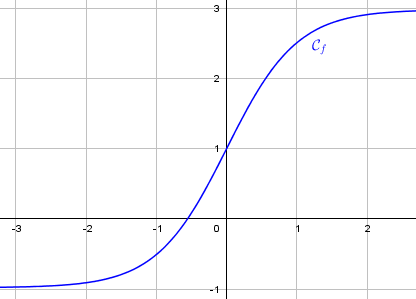
\includegraphics[scale=0.5]{media/media/image3.png}
\end{minipage}

\subsection{\textcolor{vert}{\underline{Asymptote horizontale}}}

\begin{definition}
Soit $f$ une fonction définie sur un intervalle $I$ et
$\mathscr{C}_f$ sa courbe représentative dans un repère. \par
Si la fonction $f$ admet une limite finie $L$ en $+ \infty$ (respectivement $- \infty$), alors on dit que la droite $d$ d'équation $y = L$ est une \textbf{asymptote horizontale} à la courbe $\mathcal{C}$ en $+ \infty$ (resp. $- \infty)$.
\end{definition}

\bigskip

\textbf{\underline{Remarque :}} Donner une interprétation graphique d'une limite
revient à déterminer les éventuelles asymptotes.

\bigskip

\textbf{\underline{Exemple 1 :}} On reprend l'exemple de la partie 1. Déterminer les asymptotes pour la courbe de la fonction~$f$.

\vspace{3cm}

\textbf{\underline{Exemple 2 :}} Soit une fonction $g$ définie sur $\mathbb{R}$ telle que $\displaystyle{\lim_{x \to +\infty} g(x) = 4}$ et $\displaystyle{\lim_{x \to -\infty} g(x) = -2}$. \par 
On note $\mathscr{C}_g$ la représentation graphique de la fonction $g$. \par 
Donner une interprétation graphique des limites précédentes.

\newpage 

\section{\textcolor{red}{\underline{Limite infinie en un point}}}

\subsection{\textcolor{vert}{\underline{Définitions et notations}}}

\subsection{\textcolor{vert}{\underline{Asymptote verticale}}}

\end{document}

\textbf{{Remarque~:}} Donner une interprétation graphique d'une limite
revient à déterminer les éventuelles asymptotes.

\textbf{{Exemple~1 :} }

On reprend l'exemple de la partie 1. Déterminer les asymptotes pour la
courbe de la fonction $f$.

\textbf{{Exemple~2 :} }

Soit une fonction $g$ définie sur $\mathbb{R}$ telle que
$\operatorname{}{g( x ) = \ 4}$ et
$\operatorname{}{g( x ) = \  - 2}$. On note $C_{g}$ la
représentation graphique de la fonction $g$. Donner une interprétation
graphique de ces limites.

{3 -- Notion de limite infinie en un point -- Asymptote verticale}

\begin{longtable}[]{@{}l@{}}
\toprule
\endhead
\begin{minipage}[t]{0.97\columnwidth}\raggedright
\textbf{{Définition~:}}

Soit $f$ une fonction définie sur un intervalle $I$ de la forme
$\rbrack a\ ;b\rbrack$ ou $\lbrack b\ ;a\lbrack.$

\begin{itemize}
\item
  On dit que $\mathbf{f(x)}$ \textbf{tend vers} $\mathbf{+ \infty}$
  \textbf{lorsque} $\mathbf{\text{x\ }}$\textbf{tend vers}
  $\mathbf{a}$ lorsque $f( x )\ $est aussi grand que l'on
  veut dès que $x$ est {assez proche de} $a$. On note .
\item
  On définit de façon analogue~:
\end{itemize}\strut
\end{minipage}\tabularnewline
\bottomrule
\end{longtable}

\textbf{Remarque~:} Dire que «~$f( x )\ $est aussi grand
que l'on veut dès que $x$ est {assez proche de} $a$ » signifie que
pour tout entier naturel $k$, on peut rendre
$f( x ) > 10^{k}$pour tout $x$ de $I$ suffisamment
proche de $\text{a~}$.

\begin{longtable}[]{@{}l@{}}
\toprule
\endhead
\begin{minipage}[t]{0.97\columnwidth}\raggedright
\textbf{{Définition~:}}

Si $f$ admet une limite infinie en $a$ ($a^{+}$ ou $a^{-}),$ la
droite $D$ d'équation $x = a$ est une asymptote verticale à $C$,
c'est-à-dire parallèle à l'axe des ordonnées.\strut
\end{minipage}\tabularnewline
\bottomrule
\end{longtable}

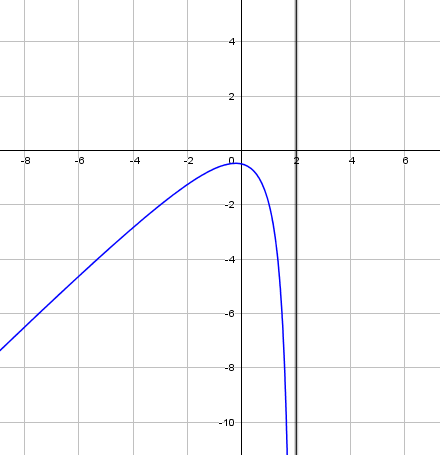
\includegraphics[width=2.08333in,height=2.12862in]{media/media/image6.png}\textbf{{Exemple~:}}
~; $D_{f} = \rbrack - \infty\ ;\ 2\lbrack.$

\begin{quote}
Soit $C$ la courbe représentative de $f$ dans le repère ci-contre.

$D$ est une asymptote horizontale à $C$.

Compléter~:

Equation de la droite $\text{D~}$:
\end{quote}

{4 --Limite infinie en l'infini}

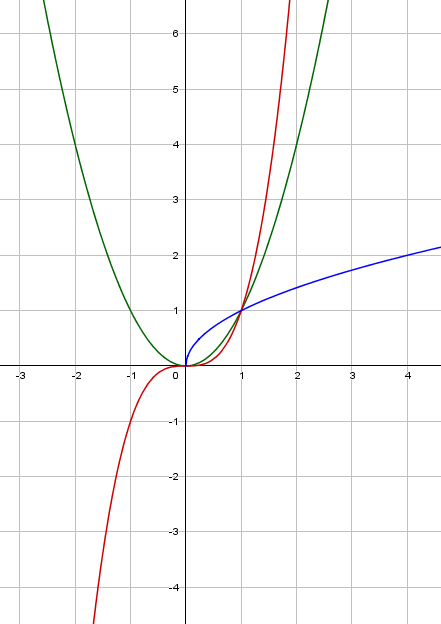
\includegraphics[width=2.95203in,height=4.17702in]{media/media/image9.png}

\begin{longtable}[]{@{}lllll@{}}
\toprule
\endhead
$x$ & & & &\tabularnewline
& & & &\tabularnewline
& & & &\tabularnewline
& & & &\tabularnewline
\bottomrule
\end{longtable}

On peut rendre $f( x )$ aussi grand que l'on veut dès que
l'on choisit $x$ suffisamment grand. (où $f$ est la fonction carré,
la fonction cube ou encore la fonction racine).

; ; ;

;

\begin{longtable}[]{@{}l@{}}
\toprule
\endhead
\begin{minipage}[t]{0.97\columnwidth}\raggedright
\textbf{{Définition~:}}

Soit $f$ une fonction définie sur un intervalle
$I = \ \rbrack a\ ;\  + \infty\ \lbrack.$

Si pour tout entier naturel $k$, on peut rendre
$f( x ) > 10^{k}$ en prenant $x$ supérieur à un certain
seuil alors on dit que $f(x)$ tend vers $+ \infty$ et on note
.\strut
\end{minipage}\tabularnewline
\bottomrule
\end{longtable}

On définira de la même façon~: ; et .

\subsection{\textcolor{vert}{\underline{Asymptote horizontale}}}





\end{document}
